\documentclass{beamer}

\usepackage[english]{babel}
\usepackage{amsmath,amsthm,amsfonts}
\usepackage{xkeyval}
\usepackage{graphics}
\usepackage{float}
\usepackage{url}
\usepackage[lined,boxed,linesnumbered]{algorithm2e}
\usepackage{CJKutf8}

\definecolor{mycolor}{RGB}{153,50,204}
\definecolor{mycolorlys}{RGB}{148,0,211}
\definecolor{mycolorlyslys}{RGB}{138,43,226}
\definecolor{mycolorlyslyslys}{RGB}{147,112,219}

%输入罗马数字
\newcommand{\myRoman}[1]{\uppercase\expandafter{\romannumeral#1}}
\newcommand{\myroman}[1]{\romannumeral#1}

\mode<presentation>
{
	\usetheme{Madrid}
	\usecolortheme[named=mycolor]{structure}
	\useinnertheme{rectangles}
	\useoutertheme{infolines}%default,infolines,miniframes,shadow,sidebar,smoothbars,smoothtree,split,tree
	\usefonttheme[onlymath]{serif}
	\setbeamercovered{transparent}
	\setbeamertemplate{blocks}[rounded][shadow=true]
}

\title{Report on UFLDL-Part \myRoman{1}}
\author{Yunfei WANG}
\institute{\inst{1}School of Computer Science \& Technology \\ Huazhong University of Science \& Technology}
\date{June 4th, 2013}
%\logo{
\includegraphics[scale=0.07]{images/HUSTLogo}}

\begin{document}
\begin{CJK*}{UTF8}{gbsn}

\begin{frame}
\titlepage
\end{frame}

\begin{frame}\frametitle{Table of contents}
\tableofcontents
\end{frame}

\section{Neural Network}
\subsection{Forward Propagation}
\begin{frame}\frametitle{Forward Propagation}
\begin{figure}
\centering
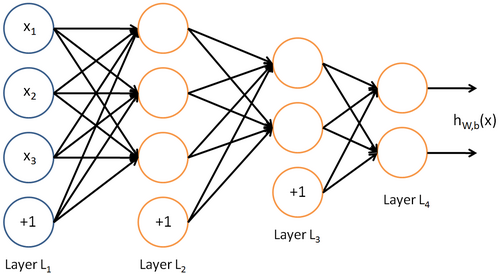
\includegraphics[scale=0.2]{images/Network}
\caption{Neural Network}
\end{figure}
\begin{block}{Forward Propagation}
\textcolor{red}{Compute activation of units one layer after another:}\\
\begin{equation}
\begin{split}
&z^{l+1}=W^la^l+b^l\\
&a^{l+1}=f(z^{l+1})
\end{split}
\end{equation}
where $z_i^l$ is weighted sum of inputs to unit $i$ in layer $l$,$a_i^l$ denotes activation of unit $i$ in layer $l$.
\end{block}
\end{frame}

\section{Back Propagation}
\begin{frame}\frametitle{Back Propagation}
\begin{exampleblock}{Cost Function for a single sample}
Measure the divergence between output and ideal targets.
\begin{equation}
J(W,b;x,y)=\frac{1}{2}\|h_{W,b}(x)-y\|^2
\end{equation}
\end{exampleblock}
\begin{exampleblock}{Overall Cost Function}
\begin{equation}
\begin{split}
J(W,b)=&\underbrace{\left[\frac{1}{m}\sum_{i=1}^mJ(W,b;x_i,y_i)\right]}_{\textcolor{red}{Mean\;Square\; Error}}+\underbrace{\frac{\lambda}{2}\sum_{l=1}^{L-1}\sum_{i=1}^{n_l}\sum_{j=1}^{n_{l+1}}(W_{ji}^l)^2}_{\textcolor{blue}{Weight\;Decay}}\\
&\left[\frac{1}{m}\sum_{i=1}^m(\frac{1}{2}\|h_{W,b}(x_i)-y_i\|^2)\right]+\frac{\lambda}{2}\sum_{l=1}^{L-1}\sum_{i=1}^{n_l}\sum_{j=1}^{n_{l+1}}(W_{ji}^l)^2
\end{split}
\end{equation}
\end{exampleblock}
\end{frame}

\subsection{Optimization Algorithm}
\begin{frame}\frametitle{Optimization Algorithm}
$J(W,b)$ is a non-convex function,\textcolor{blue}{gradient descent} is susceptible to local optima. In practice,it usually works fairly well.\\
\begin{equation}
W_{ij}^l=W_{ij}^l-\alpha\frac{\partial J(W,b)}{\partial W_{ij}^l}
\end{equation}
\begin{equation}
b_{i}^l=b_{i}^l-\alpha\frac{\partial J(W,b)}{\partial b_{i}^l}
\end{equation}

\begin{alertblock}{Derivative of overall cost function}
\begin{equation}
\frac{\partial}{\partial W_{ij}^l} J(W,b)=\left[\frac{1}{m}\sum_{i=1}^m\frac{\partial}{\partial W_{ij}^l} J(W,b;x_i,y_i)\right]+\lambda W_{ij}^l
\end{equation}
\begin{equation}
\frac{\partial}{\partial b_{i}^l} J(W,b)=\frac{1}{m}\sum_{i=1}^m\frac{\partial}{\partial b_{i}^l} J(W,b;x_i,y_i)
\end{equation}
\end{alertblock}
\end{frame}

\subsection{Processing a single sample}
\begin{frame}\frametitle{Processing a single sample}
\begin{itemize}
\item Define local gradient for simplicity:
\begin{equation}
\delta_i^l=\frac{\partial}{\partial z_i^{l}}J(W,b;x,y)
\end{equation}
\item Partial derivatives with respect to weights:
\begin{equation}
\frac{\partial J(W,b;x,y)}{\partial W_{ij}^l}=\frac{\partial J(W,b;x,y)}{\partial z_i^{l+1}}\frac{\partial z_i^{l+1}}{\partial W_{ij}^l}=\delta_{i+1}a_j^l
\end{equation}
\item Partial derivatives with respect to biases:
\begin{equation}
\frac{\partial J(W,b;x,y)}{\partial b_{i}^l}=\frac{\partial J(W,b;x,y)}{\partial z_i^{l+1}}\frac{\partial z_i^{l+1}}{\partial b_{i}^l}=\delta_{i+1}
\end{equation}
\end{itemize}
\end{frame}

\subsection{Algorithm Description}
\begin{frame}\frametitle{Single sample based gradient descend}
\begin{algorithm}[H]
%\caption{Gradient descend based on single sample}
Perform forward propagation to compute activations for all layers\;
For each unit $i$ in output layer $L$:
\begin{equation}
\delta_i^{L}=\frac{\partial}{\partial z_i^{L}}\frac{1}{2}\|y-h_{W,b}(x)\|^2=(a_i^{L}-y_i)\cdot f'(z_i^{L})
\end{equation}
\For{$l=L-1,L-2,\cdots,2$}
{
    For each unit $i$:$\delta_i^l=(\sum_{j=1}^{n_{l+1}}W_{ji}^l\delta_j^{l+1})f'(z_i^l)$\;
}
Compute corresponding partial derivatives:
\begin{equation}
\frac{\partial}{\partial W_{ij}^l}J(W,b;x,y)=a_j^l\delta_i^{l+1}
\end{equation}
\begin{equation}
\frac{\partial}{\partial b_{i}^l}J(W,b;x,y)=\delta_i^{l+1}
\end{equation}
\end{algorithm}
\end{frame}

\begin{frame}\frametitle{Vectorized Gradient Descend for single sample}
\begin{algorithm}[H]
Perform forward propagation to compute activations for all layers\;
For output layer $L$:
\begin{equation}
\delta^{L}=(a^{L}-y)\bullet f'(z^{L})
\end{equation}
\For{$l=L-1,L-2,\cdots,2$}
{
    $\delta^l=((W^l)^T\delta^{l+1})\bullet f'(z^l)$\;
}
Compute corresponding partial derivatives:
\begin{equation}
\nabla_{W^l}J(W,b;x,y)=\delta^{l+1}(a^l)^T
\end{equation}
\begin{equation}
\nabla_{b^l}J(W,b;x,y)=\delta^{l+1}
\end{equation}\;
\end{algorithm}
\end{frame}

\begin{frame}\frametitle{Batch Gradient Descendent}
\begin{figure}
\centering
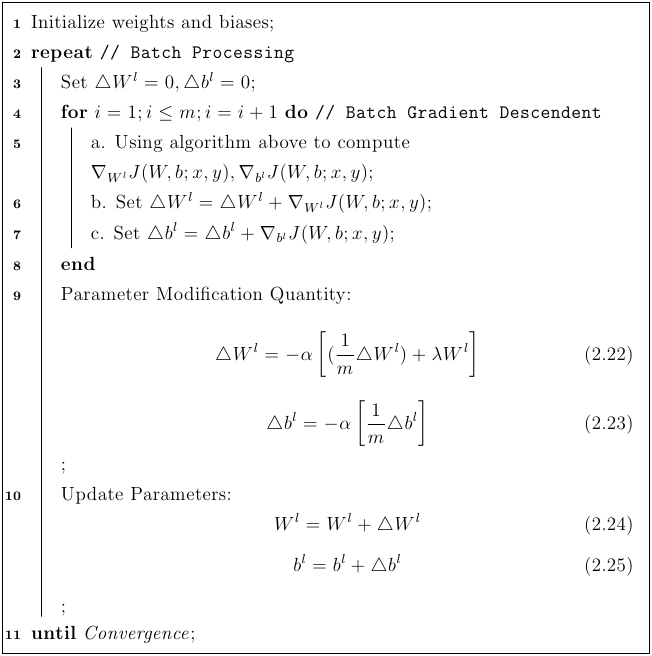
\includegraphics[scale=0.32]{images/algorithm}
\end{figure}
\end{frame}

\subsection{Momentum}
\begin{frame}\frametitle{Momentum}
\textcolor{blue}{Momentum} is used to accelerate learning procedure:
\begin{equation}
\bigtriangleup W^l(t+1)=\tau\bigtriangleup W^l(t)-\alpha\nabla_{W^l}J(W,b;x,y)
\end{equation}
$\nabla_{W^l}J(W,b;x,y)$ is fixed here,a brief explanation for acceleration of momentum is provided below($\tau\in[0.9\sim 1)$):

\end{frame}

\section{Autoencoder}
\subsection{Sparsity Constraint}
\begin{frame}\frametitle{Sparsity Constraint}
Average activation of hidden unit $j$ in layer $l$:
\begin{equation}
\rho_j^l=\frac{1}{m}\sum_{i=1}^m\left[a_j^l(x_i)\right]
\end{equation}
KL-divergence is used to force $\rho_j^l=\rho$($\rho$ is a small sparsity parameter):
\begin{equation}
KL(\rho||\rho_j^l)=\rho\log\frac{\rho}{\rho_j^l}+(1-\rho)\log\frac{1-\rho}{1-\rho_j^l}
\end{equation}
Add extra sparsity penalty term to achieve sparsity constraint:
\begin{equation}
\sum_{j=1}^{s_2}KL(\rho||\rho_j^l)=\sum_{j=1}^{s_l}\rho\log\frac{\rho}{\rho_j^l}+(1-\rho)\log\frac{1-\rho}{1-\rho_j^l}
\end{equation}
\end{frame}

\subsection{Objective Function}
\begin{frame}\frametitle{Objective Function of Autoencoder}
Our overall objective function is:
\begin{equation}
J_{sparse}(W,b)=J(W,b)+\beta\sum_{l=2}^{L-1}\sum_{i=1}^{s_l}KL(\rho||\rho_i^l)
\end{equation}
where $J(W,b)$ is defined as previous,$\beta$ controls weight of sparsity penalty term,$\rho_j^l$ implicitly depends on $W,b$.\\
\bigskip
Make small change to the algorithm above to incorporate KL-divergence term into derivative calculation:
\begin{equation}\label{eq:deltasparse}
\delta_i^l=\left(\left(\sum_{j=1}^{s_l}W_{ji}^l\delta_j^{l+1}\right)+\beta\left(-\frac{\rho}{\rho_i^l}+\frac{1-\rho}{1-\rho_i^l}\right)\right)f'(z_i^l)
\end{equation}
\end{frame}

\subsection{Derivation}
\begin{frame}[allowframebreaks]\frametitle{Simple Derivation}
For simplicity,we divide the sparsity penalty term into small items:
\begin{equation}
S=\beta\sum_{l=2}^{L-1}S^l
\end{equation}
where $S^l$ is sparsity penalty term for layer $l$:
\begin{equation}
\begin{split}
S^l&=\sum_{i=1}^{s_l}KL(\rho||\rho_i^l)\\
&=\sum_{i=1}^{s_l}\left[\rho(\log\rho-\log\rho_i^l)+(1-\rho)(\log(1-\rho)-\log(1-\rho_i^l))\right]
\end{split}
\end{equation}
It's apparent that $J_{sparse}(W,b)=J(W,b)+S$.\\
Next,we have the following partial derivatives:
\begin{equation}
\frac{\partial S^l}{\partial\rho_i^l}=\frac{KL(\rho||\rho_i^l)}{\partial\rho_i^l}=-\frac{\rho}{\rho_i^l}+\frac{1-\rho}{1-\rho_i^l}
\end{equation}
\begin{equation}
\frac{\partial\rho_i^l}{\partial z_i^l}=\frac{1}{m}\frac{\sum_{j=1}^m a_i^l(x_j)}{\partial z_i^l}=\frac{1}{m}\sum_{j=1}^m f'(z_i^l(x_j))
\end{equation}
\begin{equation}
\begin{split}
\frac{\partial S}{\partial z_i^l}&=\frac{\partial S}{\partial S^l}\frac{\partial S^l}{\partial\rho_i^l}\frac{\partial\rho_i^l}{\partial z_i^l}\\
&=\beta\left(-\frac{\rho}{\rho_i^l}+\frac{1-\rho}{1-\rho_i^l}\right)f'(z_i^l)
\end{split}
\end{equation}
Based on the derivations above,we have the following equation:
\begin{equation}
\begin{split}
\frac{\partial J_{sparse}(W,b)}{\partial z_i^l}&=\frac{\partial J(W,b)}{\partial z_i^l}+\frac{\partial S}{\partial z_i^l}\\
&=\left(\left(\sum_{j=1}^{s_l}W_{ji}^l\delta_j^{l+1}\right)+\beta\left(-\frac{\rho}{\rho_i^l}+\frac{1-\rho}{1-\rho_i^l}\right)\right)f'(z_i^l)
\end{split}
\end{equation}
\end{frame}


\section{Experiments}
\begin{frame}\frametitle{What does Autoencoder learn?}
\begin{minipage}{\linewidth}
\begin{minipage}{0.5\linewidth}
\begin{figure}[H]
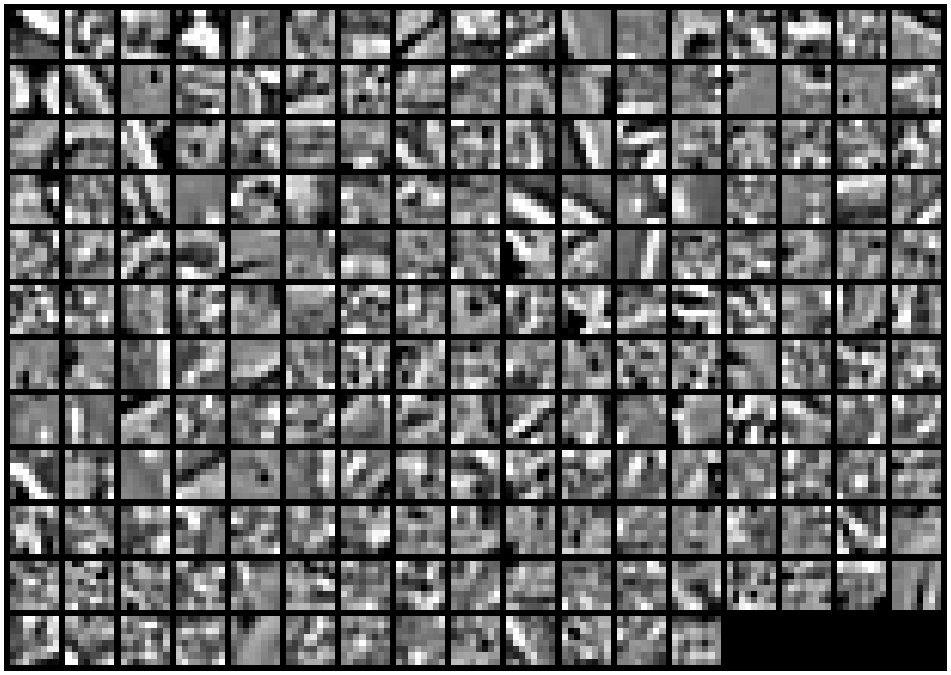
\includegraphics[scale=0.18]{images/patches}
\caption{Training Examples}
\end{figure}
\end{minipage}
\begin{minipage}{0.5\linewidth}
\begin{figure}[H]
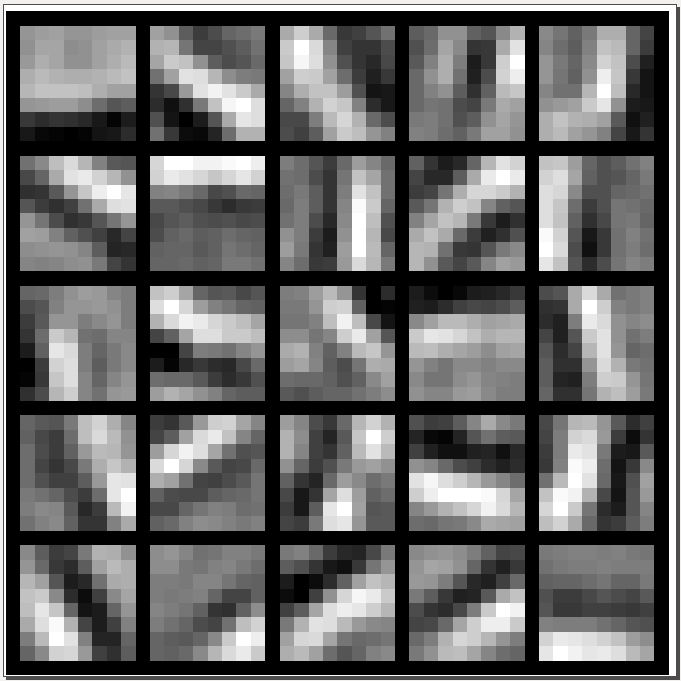
\includegraphics[scale=0.22]{images/weights}
\caption{Learned Edges}
\end{figure}
\end{minipage}
\end{minipage}
Different hidden units have learned to detect edges at different positions and orientations in the images,which are quite useful for object recognition and other vision tasks.
\end{frame}

\begin{frame}\frametitle{Trying to run faster}
\begin{minipage}{\linewidth}
\begin{minipage}{0.5\linewidth}
\begin{figure}[H]
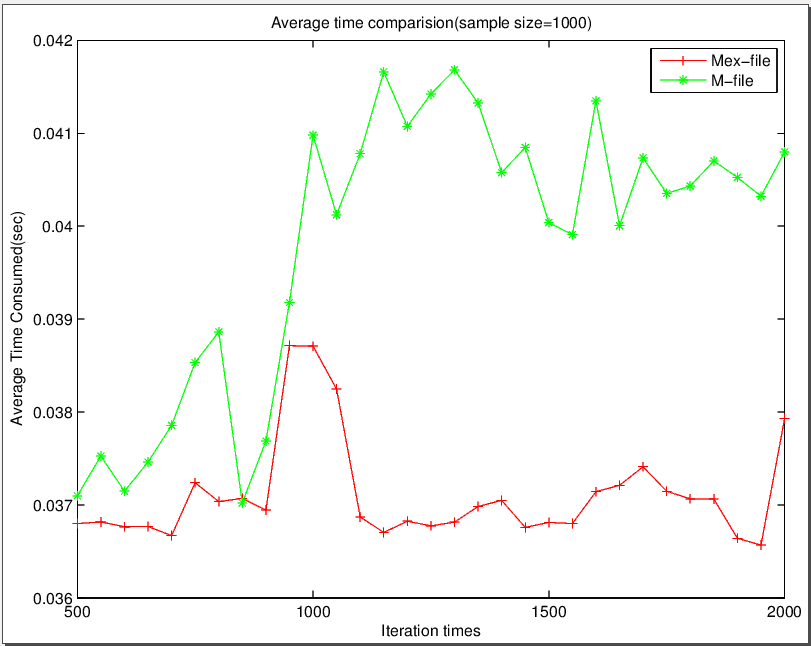
\includegraphics[scale=0.2]{images/time_test_iter}
\caption{Average Time Consumed}
\end{figure}
\end{minipage}
\begin{minipage}{0.5\linewidth}
\begin{figure}[H]
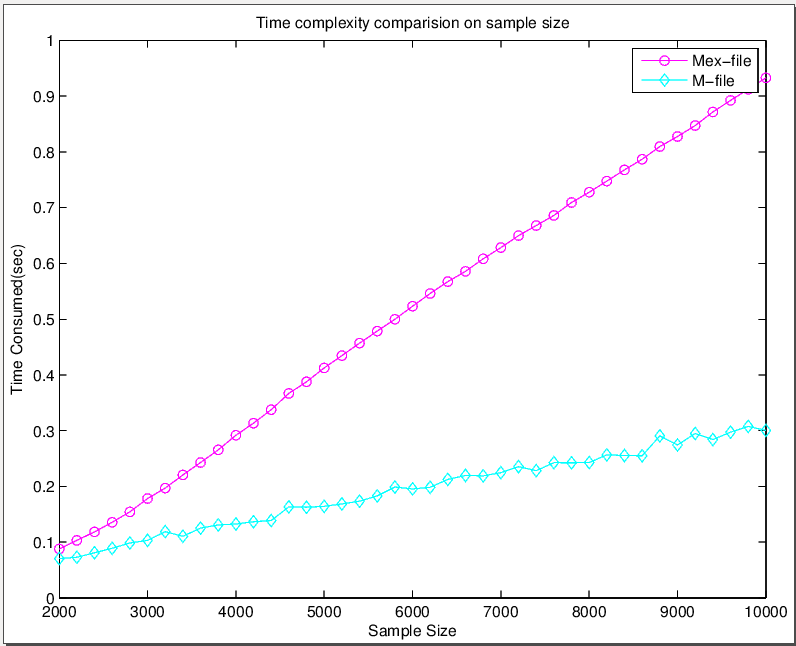
\includegraphics[scale=0.2]{images/time_test_size}
\caption{Time Consumed VS Sample Size}
\end{figure}
\end{minipage}
\end{minipage}
\end{frame}


\end{CJK*}
\end{document}
